\section{背景与动机}
\label{sec:background}
\subsection{LFM 开发}\label{sec:bg_lfm}

 \begin{figure}[!t]
  \centering
  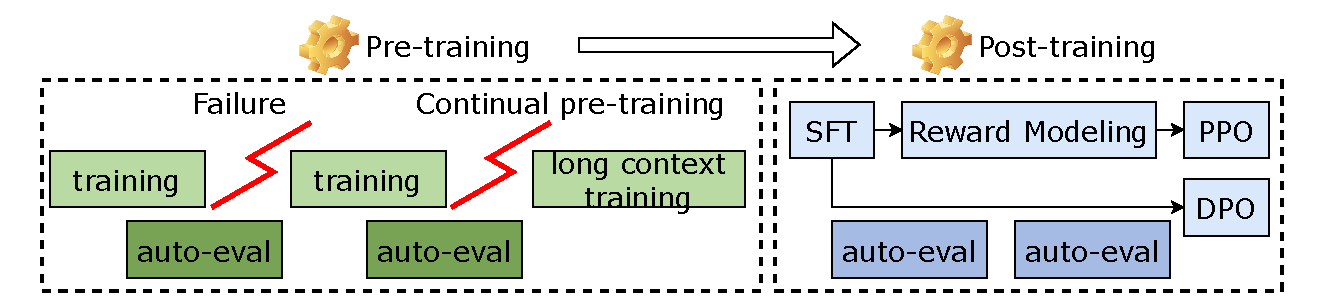
\includegraphics[width=0.95\linewidth]{figures/lfm_pipeline.pdf}
  \caption{
  LFM 训练流水线概览。
  }
  \label{fig:lfm_pipeline}
  \vspace{-3mm}
\end{figure}

\noindent \textbf{生产流水线}。
如图~\ref{fig:lfm_pipeline} 所示，LFM 的开发包含 pre-training 与 post-training 阶段。
在初始 pre-training 阶段，LFM 在来自多源的大规模数据上迭代训练，以吸收世界知识。
随后，通过持续 pre-training 进一步增强基础模型能力。
例如，大语言模型（LLM）的 pre-training 通常会进行长上下文持续训练，以逐步提升模型支持的 context length。
post-training 用于对齐人类反馈或提升模型推理能力~\cite{openai-o1, deepseek-r1}。
在 fine-tuning 中会使用多种任务特定的标注数据集（\eg，多语种、代码、数学、推理等），随后进行强化学习，通常包括 reward modeling 与 Proximal Policy Optimization（PPO）~\cite{ppo}，或直接进行 Direct Preference Optimization（DPO）~\cite{dpo}。
由于这些数据集规模较小，post-training 通常使用更少的 GPUs。
在这些阶段中，还会周期性触发自动评测~\cite{characterization, check-n-run}，拉取中间 checkpoints 并通过多维度指标评估模型质量。

\noindent \textbf{Checkpointing}。
LFM 训练任务的训练状态包括 GPU 与 CPU 状态。
GPU 状态是 LFM 的可学习参数以及优化器信息（例如 Adam~\cite{adam} 中模型的 float32 精度副本及其动量与方差）。
在最先进的大规模并行训练~\cite{megatron-lm3} 中，这些状态会被分片并分布在多张 GPU 上。
CPU 状态包括 dataloader 模块、随机数生成器（RNG）状态、全局训练步数以及学习率调度器等，均存放在 CPU 内存。
我们的 dataloader 模块包含 token buffer，用于缓存来自数据源的不同长度样本；当累计 token 数达到 context window size~\cite{megascale, llama3.1, opt, glm} 时，dataloader 会将缓存样本组装成一个 batch（micro-batch）。
由于 GPU 与 CPU 内存具备易失性，这些训练状态需要周期性保存到持久化存储，以容忍故障并支撑 evaluation 任务。

\noindent \textbf{Storage backends}。
在生产环境中，训练通常使用独立的分布式文件系统（如 Llama 3.1 训练使用的 Tectonic~\cite{tectonic}~\cite{llama3.1}）存储 checkpoints~\cite{check-n-run, unicron}。
鉴于训练中不可避免的硬件故障与软件缺陷~\cite{llama3.1, megascale,characterization}，必须在不同训练步上保存 checkpoints 以保障训练安全。
分布式文件系统（如 HDFS、NAS）提供充足的存储容量，以容纳大型模型的多个 checkpoints。

\subsection{Checkpoint Resharding 场景}\label{sec:bg_ckpt}

\begin{figure}[!t]
  \centering
  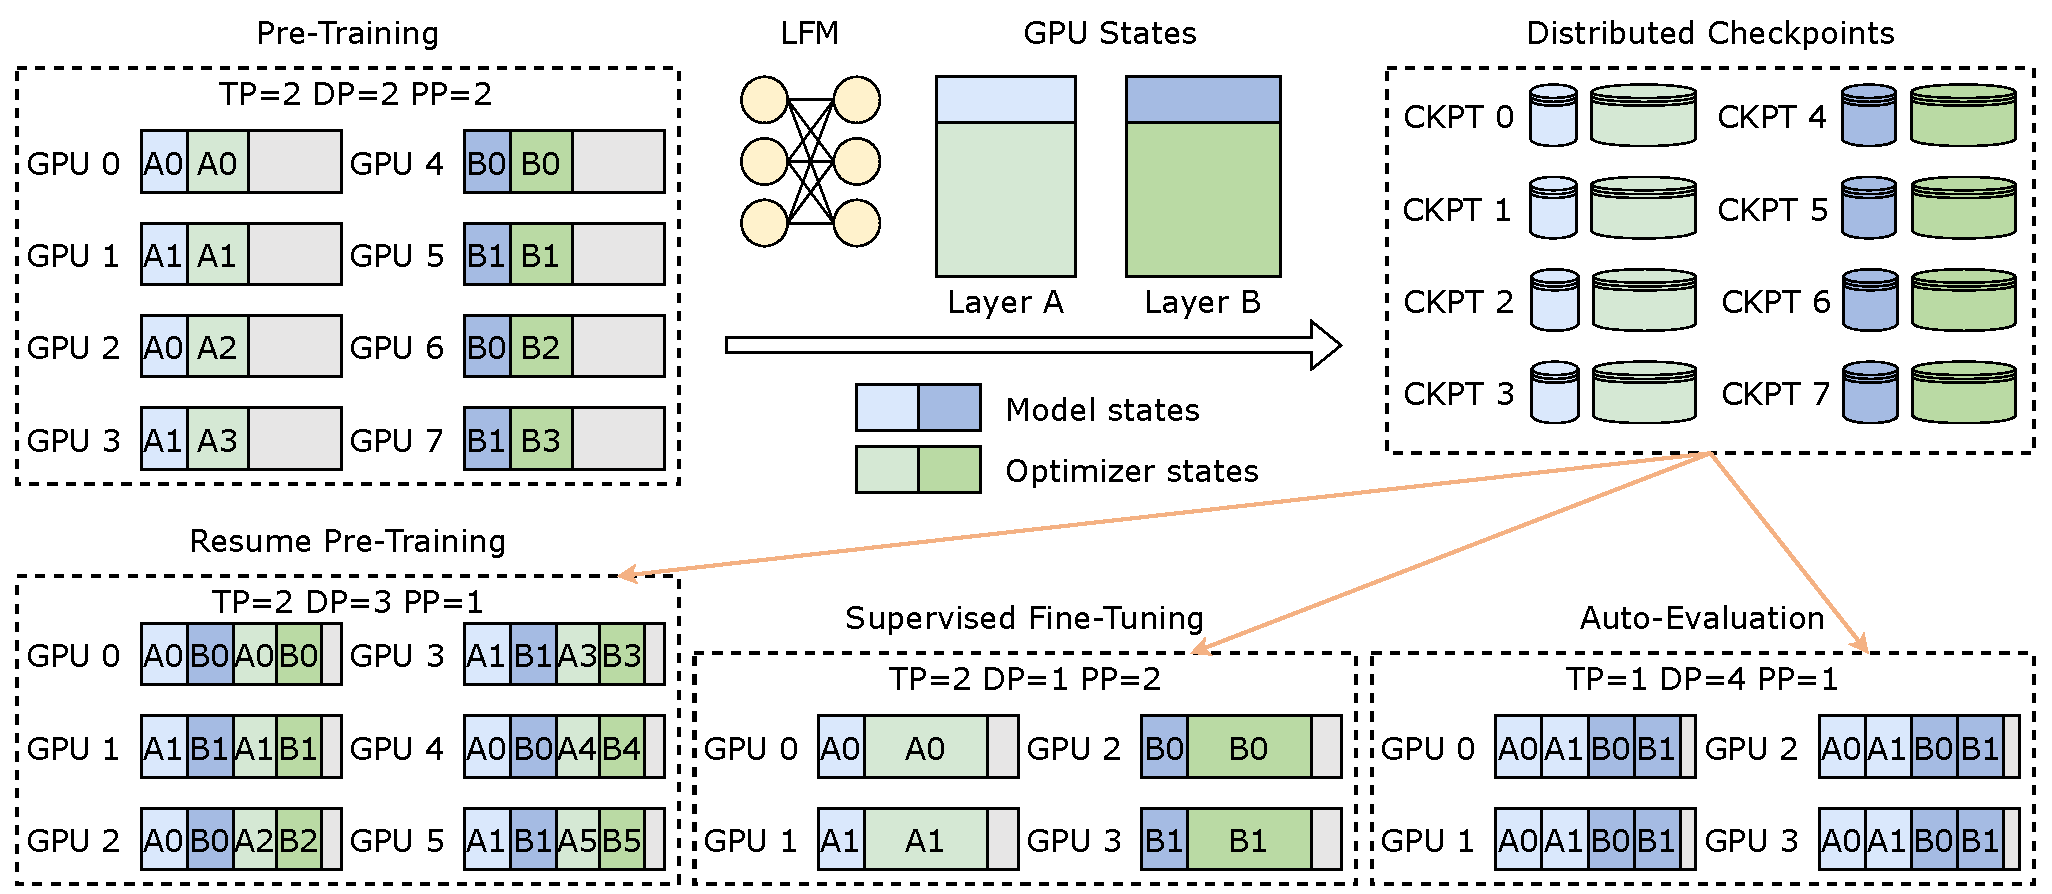
\includegraphics[width=\linewidth]{figures/resharding_requirements.pdf}
  \caption{LFM 训练中的 checkpoint resharding 场景。
  为便于展示，图中仅绘制 GPU 状态。
  }
  \label{fig:reshard_req}
\end{figure}

在 LFM 开发生命周期中，parallelism 在不同场景下发生变化，因此 checkpoint resharding 持续存在（图~\ref{fig:reshard_req}）：

\noindent \textit{(1) 训练恢复}。
LFM 训练任务的 GPU 配额可能因故障机器移除~\cite{megascale, characterization}、新增可用机器，或使用潮汐资源~\cite{parcae, qsync, lyra, antman}而发生变化。
为了最大化资源利用率，往往需要据此调整训练 parallelism。
此外，在大规模 pre-training 初期，工程师通常需要探索不同模型配置与优化技术~\cite{megascale}，因为小规模 profile 或仿真结论未必适用于大规模训练。
在这一阶段，parallelism 配置频繁调整，导致训练反复恢复。
此外，长上下文训练会改变 context length，也会引发 GPU 配额或 parallelism 调整。
如图~\ref{fig:reshard_req} 所示示例，最初保存了 8 个分布式 checkpoint 文件，恢复时加载到 6 个训练 worker。

\noindent \textit{(2) 跨阶段切换}。
进入 post-training 阶段时，因后续训练数据规模更小，参与训练的 GPU 数量通常降低。
pre-training 保存的 checkpoints 需要 resharding 以适配各类 post-training 任务的具体工作负载。
如图~\ref{fig:reshard_req} 所示，post-training 的 fine-tuning 任务仅使用 4 GPUs，因此需要将 checkpoints 进行相应 resharding。

\noindent \textit{(3) 评测}。
两个阶段的 evaluation 任务都需要加载模型 checkpoints 并在独立资源上进行推理；其 parallelism 需与评测任务分配的 GPU 资源匹配。
图~\ref{fig:reshard_req} 展示了一个 4-GPU 的评测任务从 pre-training checkpoints 进行 resharding 的场景。

我们统计了平台最近六个月（训练文本、图像与视频生成模型）的 resharding 需求：pre-training 恢复场景 1,870 次，跨阶段重配置 13,080 次，评测任务 19,844 次。


\subsection{LFM Checkpointing 需求}\label{sec:bg_challenges}
\noindent \textbf{Load-time checkpoint resharding}。
作为 LFM 开发生命周期中的关键步骤，checkpoint resharding 的效率决定了额外开销的大小。
在我们的 AI 平台上，过去的常见做法是编写离线 resharding 脚本，并在出现新 resharding 场景时调整脚本。
该方法低效且人力成本高（详见附录~\ref{sec:reshard_scripts}）。
除了开发成本，离线脚本运行还会浪费大量 GPU 时间与资源。
表~\ref{tab:resharding_duration} 给出了不同场景下离线 resharding 作业的开销。
在训练恢复或评测开始之前，必须先提交独立作业执行 resharding：从存储系统下载 checkpoints，按指定 parallelism 进行 resharding，再上传到存储系统。
目标训练或评测作业在 resharding 作业完成前无法启动，导致等待时间延长。
此外，离线脚本生成的 checkpoints 与特定 parallelism 绑定，难以复用，增加了存储开销。

相比之下，\textit{load-time checkpoint resharding}~\cite{torch-dcp}（也称在线 resharding）更适合 LFM 训练。
它在加载阶段自动识别并从现有分布式 checkpoints 中提取所需数据。
要实现这一点，checkpoint 的存储表示必须与具体 parallelism 解耦。

% \subsubsection{Supporting multiple training frameworks \& storage backends}
\begin{table}[!t]
\caption{
不同场景下离线 resharding 作业的平均完成时间。
}
\label{tab:resharding_duration}
\resizebox{\linewidth}{!}{
\begin{tabular}{ccc}
    \toprule
    \textbf{Training Resumption} &  \textbf{Cross-Stage Transition} & \textbf{Evaluation}   \\
    \midrule
     1870.38s & 650.34s & 593.21s\\
    \bottomrule
\end{tabular}}
\end{table}

\begin{table}[!t]
\caption{平台上使用最广泛的三类训练框架
}
\label{tab:framework_distribute}
\resizebox{\linewidth}{!}{
\begin{tabular}{cccc}
    \toprule
    \textbf{Framework} & \textbf{Pre-training} &  \textbf{Post-training} & \textbf{Average \#GPUs Per Job}
    \\
    \midrule
    Megatron-LM & 13727& 68621& 301\\
    FSDP & 16842 & $\dagger$ &  25\\
    DDP & 25393& $\dagger$&  6\\
    \bottomrule
\end{tabular}}
\end{table}

\noindent \textbf{多训练框架与多 storage backend}。
我们的 AI 平台上使用了多种训练框架，如 Megatron-LM~\cite{megatron}、DDP~\cite{ddp}、FSDP~\cite{fsdp}、veScale~\cite{megascale, vescale} 等。
表~\ref{tab:framework_distribute} 基于六个月的轨迹分析给出了平台上最常用的三类训练框架。
用户通常使用 Megatron-LM~\cite{megatron} 训练大型语言基础模型。
FSDP~\cite{fsdp} 常用于 text-to-video 或 text-to-speech 模型训练，
而 DDP~\cite{ddp} 则多用于多模态基础模型中的图像编码器训练或日常算法测试。
此外，用户还可根据场景选择不同 storage backend 保存 checkpoints，从调试时的本地磁盘到正式训练时的 HDFS 或 NAS。

每种训练框架都自带 checkpoint 模块、文件格式与保存/加载逻辑的临时实现。
然而这些模块缺乏生产级能力，如 load-time resharding、异步 checkpointing、以及对远程持久化存储的支持。
针对每个框架单独补齐这些能力并实现优化，意味着重复的工程成本，也造成跨框架/存储 backend 的接口不一致，增加代码复杂度。
同时，不同框架的 checkpoint 文件格式差异也增加了跨阶段 checkpoint 转移与评测/推理部署的复杂度。
因此，需要为不同训练框架与 storage backend 提供通用 workflow。

\begin{figure}[!t]
  \centering
  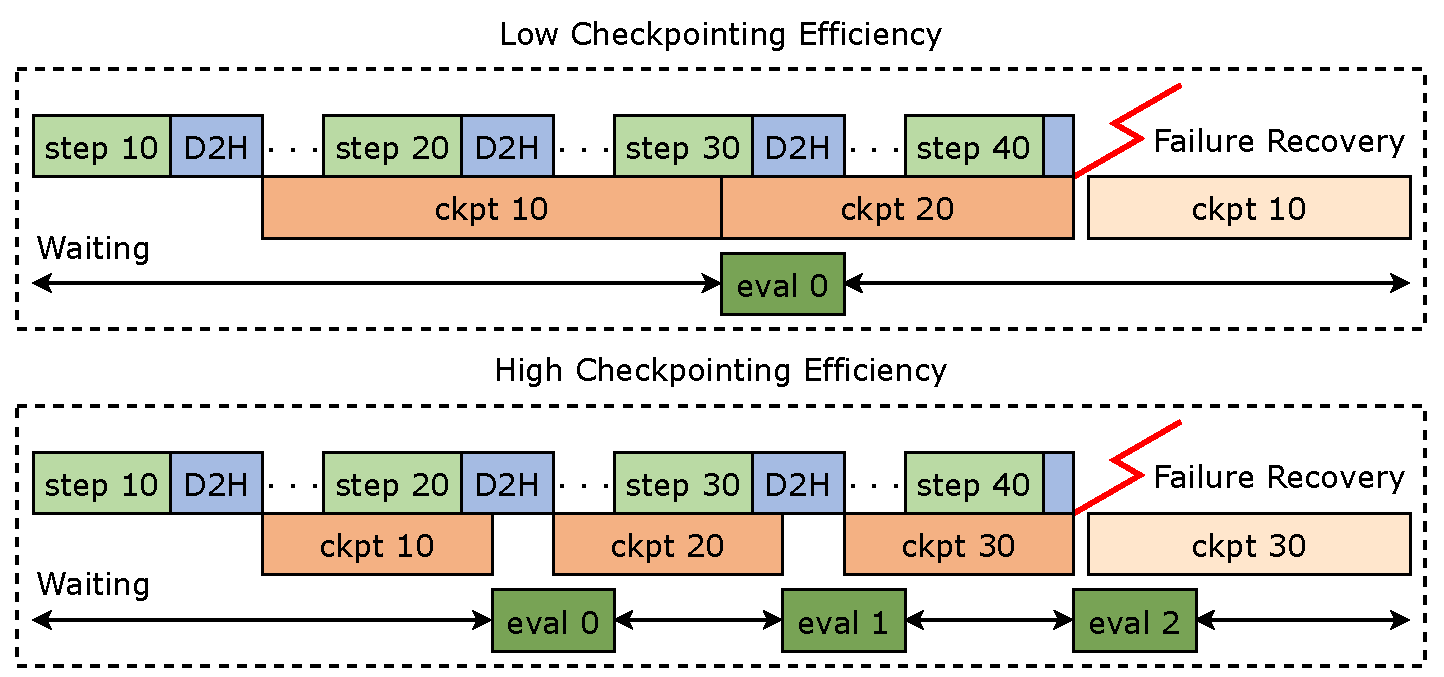
\includegraphics[width=\linewidth]{figures/checkpoint_efficiency.pdf}
  \caption{
  Checkpointing 效率对故障恢复与评测任务的影响。
  D2H 表示 Device-to-Host 拷贝。
  }
  \label{fig:check_efficiency}
  \vspace{-5mm}
\end{figure}

\noindent \textbf{高效且可扩展的 I/O 性能}。
主流 LFM 模型规模巨大，可达数千亿参数~\cite{llama3.1}。
因此训练状态大小也显著增加，带来 checkpoint 保存与加载的巨大开销。
基于我们对历史 LFM 训练任务的分析，4096 GPUs 训练的 GPT-175B 模型，其分布式 checkpoints 写入 HDFS 的平均端到端时间可达 200 秒，远超单次训练迭代时间。
尽管采用异步 checkpointing~\cite{checkfreq, megascale, reft, datastates-llm} 能将一部分开销移出训练关键路径，但端到端 checkpointing 的加速仍至关重要，可在不可避免的频繁故障~\cite{megascale} 中减少训练进度损失~\cite{gemini-sys}。
如图~\ref{fig:check_efficiency} 所示，即使 checkpointing 与训练并行进行，若能更快完成，就能在故障前保存更多中间 checkpoints，从而恢复到更近的状态并提升 ETTR。
此外，训练过程中会触发 evaluation 任务并周期性拉取中间 checkpoints，checkpointing 越快，评测准备阻塞越少。

在保持高 I/O 性能的同时进行规模扩展并不容易。
一些在小规模下难以发现的次优或高风险设计，可能在大规模训练中导致严重性能瓶颈甚至灾难性作业失败。
例如，训练集群到存储系统（如 HDFS）的海量读写请求可能压垮 master 节点，导致文件元数据操作延迟。
此外，朴素的集体通信实现（如完整性检查 barrier）会引入显著的初始化与同步开销，甚至触发通信超时，从而导致训练失败。
随着规模增长，在跨多机的训练与 I/O worker 间高效分析性能与检测错误也愈加困难。

现有 checkpointing 系统（如 CheckFreq~\cite{checkfreq}、Check-N-Run~\cite{check-n-run}、Gemini~\cite{gemini-sys}）都假设 parallelism 不变，无法满足 resharding 需求。
DCP~\cite{torch-dcp} 与 MCP~\cite{torch-dcp} 虽具备 resharding 能力，但在并行策略/框架支持、I/O 性能与可扩展性方面仍受限。
我们在附录~\ref{sec:related_work} 对相关工作进行了更全面讨论。
在 \sys{} 中，我们设计了与 parallelism 解耦的存储表示来支持高效 load-time resharding，提出通用保存/加载 workflow 以支持多框架与多 storage backend，并集成 full-stack 优化以提升 I/O 性能，同时分享了在真实 LFM 训练中扩展 checkpointing 系统的经验。
